%%%%%%%%%%%%%%%%%%%%%%%%%%%%%%%%%%%%%%%%%%%%%%%%%%%%%%%%%%%%%%%%%%%%%%%%%%%%
% AGUJournalTemplate.tex: this template file is for articles formatted with LaTeX
%
% This file includes commands and instructions
% given in the order necessary to produce a final output that will
% satisfy AGU requirements, including customized APA reference formatting.
%
% You may copy this file and give it your
% article name, and enter your text.
%
%% To submit your paper:
\documentclass[draft]{jgr/agujournal2019}
\usepackage{url} %this package should fix any errors with URLs in refs.
\usepackage{lineno}
\usepackage[inline]{jgr/trackchanges} %for better track changes. finalnew option will compile document with changes incorporated.
\usepackage{soul}
\usepackage{marginnote} % comment out on submission
\linenumbers
%%%%%%%
% As of 2018 we recommend use of the TrackChanges package to mark revisions.
% The trackchanges package adds five new LaTeX commands:
%
%  \note[editor]{The note}
%  \annote[editor]{Text to annotate}{The note}
%  \add[editor]{Text to add}
%  \remove[editor]{Text to remove}
%  \change[editor]{Text to remove}{Text to add}
%
% complete documentation is here: http://trackchanges.sourceforge.net/
%%%%%%%

\draftfalse

%% Enter journal name below.
%% Choose from this list of Journals:
%
% JGR: Atmospheres
% JGR: Biogeosciences
% JGR: Earth Surface
% JGR: Oceans
% JGR: Planets
% JGR: Solid Earth
% JGR: Space Physics
% Global Biogeochemical Cycles
% Geophysical Research Letters
% Paleoceanography and Paleoclimatology
% Radio Science
% Reviews of Geophysics
% Tectonics
% Space Weather
% Water Resources Research
% Geochemistry, Geophysics, Geosystems
% Journal of Advances in Modeling Earth Systems (JAMES)
% Earth's Future
% Earth and Space Science
% Geohealth
%
% ie, \journalname{Water Resources Research}

\journalname{JGR: Oceans}


\begin{document}

%% ------------------------------------------------------------------------ %%
%  Title
%
% (A title should be specific, informative, and brief. Use
% abbreviations only if they are defined in the abstract. Titles that
% start with general keywords then specific terms are optimized in
% searches)
%
%% ------------------------------------------------------------------------ %%

\title{Microplastic Transport and Fate in Estuarine and Coastal Flows}

%% ------------------------------------------------------------------------ %%
%
%  AUTHORS AND AFFILIATIONS
%
%% ------------------------------------------------------------------------ %%

% Authors are individuals who have significantly contributed to the
% research and preparation of the article. Group authors are allowed, if
% each author in the group is separately identified in an appendix.)

% List authors by first name or initial followed by last name and
% separated by commas. Use \affil{} to number affiliations, and
% \thanks{} for author notes.
% Additional author notes should be indicated with \thanks{} (for
% example, for current addresses).

% Example: \authors{A. B. Author\affil{1}\thanks{Current address, Antartica}, B. C. Author\affil{2,3}, and D. E.
% Author\affil{3,4}\thanks{Also funded by Monsanto.}}

\authors{R. C. Holleman\affil{1}\thanks{Current address, HERE},
  R. Sutton\affil{2},
  M. Sedlak\affil{2}, 
  D. Lin\affil{2}, 
  C. Rochman\affil{3}, and
  A. Wong\affil{2} }

\affiliation{1}{Center for Watershed Sciences, University of California, Davis}
\affiliation{2}{San Francisco Estuary Institute}
\affiliation{3}{Department of Ecology and Evolutionary Biology, University of Toronto}

%% Corresponding Author:
% Corresponding author mailing address and e-mail address:

% (include name and email addresses of the corresponding author.  More
% than one corresponding author is allowed in this LaTeX file and for
% publication; but only one corresponding author is allowed in our
% editorial system.)

% Example: \correspondingauthor{First and Last Name}{email@address.edu}

\correspondingauthor{Rusty Holleman}{cdholleman@ucdavis.edu}

%% Keypoints, final entry on title page.

%  List up to three key points (at least one is required)
%  Key Points summarize the main points and conclusions of the article
%  Each must be 140 characters or fewer with no special characters or punctuation and must be complete sentences

% Example:
% \begin{keypoints}
% \item	List up to three key points (at least one is required)
% \item	Key Points summarize the main points and conclusions of the article
% \item	Each must be 140 characters or fewer with no special characters or punctuation and must be complete sentences
% \end{keypoints}

\begin{keypoints}
\item Microplastic loads from stormwater have a settling velocity distribution biased toward
  sinking relative to loads from wastewater.
\item A three-dimensional transport model predicts
  sea surface abundance of plastics with good correlation to observations but a substantial bias toward
  large abundances.
\item The estuarine circulation is highly effective at sorting paricles by settling/rising velocities such
  that only all buoyant and neutral particles exit the estuary.
\end{keypoints}

%% ------------------------------------------------------------------------ %%
%
%  ABSTRACT and PLAIN LANGUAGE SUMMARY
%
% A good Abstract will begin with a short description of the problem
% being addressed, briefly describe the new data or analyses, then
% briefly states the main conclusion(s) and how they are supported and
% uncertainties.

% The Plain Language Summary should be written for a broad audience,
% including journalists and the science-interested public, that will not have 
% a background in your field.
%
% A Plain Language Summary is required in GRL, JGR: Planets, JGR: Biogeosciences,
% JGR: Oceans, G-Cubed, Reviews of Geophysics, and JAMES.
% see http://sharingscience.agu.org/creating-plain-language-summary/)
%
%% ------------------------------------------------------------------------ %%

%% \begin{abstract} starts the second page

\begin{abstract}
  Microplastic pollution is a growing concern in surface waters, both
  inland and marine, yet the pathways between terrestrial sources and
  accumulation in open water and sediment is poorly quantified. This
  study links microplastic loads in stormwater and wastewater to
  ambient concentrations in San Francisco Bay and the coastal ocean by
  means of a three-dimensional hydrodynamic and particle tracking
  model.  Microscopy and spectoscopy data for collected particles are
  used to estimate particle settling rates. Particle tracking results
  bear out the major patterns in the observed concentrations, and
  suggests a surface persistnce time scale on the order of days,
  before particles are degraded or fouled and sink from the water
  surface. Abundance within the Bay is shown to be substantially
  higher than in the coastal ocean.  Particle buoyancy exerts a strong
  control on the fate of particles, with negatively buoyant particles
  effectively trapped within the Bay due to interactions with
  estuarine circulation.
\end{abstract}

\section*{Plain Language Summary}
Microplastic pollution consists of plastic particles less than 5 mm in
diameter. Concentrations of these particles were measured in
wastewater and stormwater flows entering San Francisco Bay. A computer
model simulated how these particles are transported by the tides and
ocean currents, and predicted concentrations of microplastics
throughout the Bay and the coastal ocean. Comparison of the model predictions
with observed concentrations show that the model can explain a substantial
amount of the observed patterns. The model also shows that almost all
sinking particles are retained inside the Bay, while some floating particles
are carried into the coastal ocean and potentially reach nearby
National Marine Sanctuaries.

%% ------------------------------------------------------------------------ %%
%
%  TEXT
%
%% ------------------------------------------------------------------------ %%

%%% Suggested section heads:
% \section{Introduction}
%
% The main text should start with an introduction. Except for short
% manuscripts (such as comments and replies), the text should be divided
% into sections, each with its own heading.

% Headings should be sentence fragments and do not begin with a
% lowercase letter or number. Examples of good headings are:

% \section{Materials and Methods}
% Here is text on Materials and Methods.
%
% \subsection{A descriptive heading about methods}
% More about Methods.
%
% \section{Data} (Or section title might be a descriptive heading about data)
%
% \section{Results} (Or section title might be a descriptive heading about the
% results)
%
% \section{Conclusions}


\section{Introduction}
  Microplastic pollution is a growing concern in surface waters, both
  inland and marine, yet the pathways between terrestrial sources and
  accumulation in open water and sediment is poorly quantified.

  Transport of microparticles and microplastics in surface waters is
  an essential component of understanding the fate of particles in the
  environment, and the degree to which microparticles entering surface
  water systems may be transported downstream and into the open
  ocean. Microplastic transport modeling in the open ocean has
  demonstrated the physical processes responsible for mid-ocean
  accumulation zones, specifically looking at surface-bound, buoyant
  particles (e.g., Lebreton et al, 2019).
  % Need a better reference here. Jambeck is about total loads, but
  % I think she stops shy of a budget
  Loading studies such as {\bf
  Jambeck et al} find that the microplastic budgets including
  estimated loads and open ocean concentrations do not close, and
  suggest large loss terms somewhere between the point of loading and
  the open ocean.

  Sutton et al.(2016) found that particles entering San Francisco Bay
  exhibited a wide variety of characteristics and likely have a wide
  range of settling velocities.  Studies of sediment transport
  dynamics suggest that transport and fate of material in an estuarine
  setting is highly dependent on settling velocities (Williams et al,
  2004), and only a fully three-dimensional analysis of transport can
  capture the breadth of relevant mechanisms (Scheu et al, 2015).
  
  This study links microplastic loads in stormwater and wastewater to
  ambient concentrations in San Francisco Bay and the coastal ocean by
  means of a three-dimensional hydrodynamic and particle tracking
  model.  Microscopy and spectoscopy data for collected particles are
  used to estimate particle settling rates. Particle tracking results
  bear out the major patterns in the observed concentrations, and
  suggests a surface persistnce time scale on the order of days,
  before particles are degraded or fouled and sink from the water
  surface. Abundance within the Bay is shown to be substantially
  higher than in the coastal ocean.  Particle buoyancy exerts a strong
  control on the fate of particles, with negatively buoyant particles
  effectively trapped within the Bay due to interactions with
  estuarine circulation.

  % Uncategorized intro material:
  \cite{Atwood2019} modeled distribution of microplastics in surface water
  and beaches around the Po River Delta using a Lagrangian particle tracking
  method. Particles were subjected to full 3D transport including thermohaline
  interaction, but only a single particle density was included (corresponding
  to virgin polyethylene).


  
\subsection{San Francisco Bay}

The study area is San Francisco Bay and the adjacent coastal ocean
including the majority of three National Marine Sanctuaries (Greater
Farallones, Cordell Bank and Monterey Bay).

% Physical setting
San Francisco Bay is a mesotidal estuary with mixed diurnal and
semidiurnal tides, and a great diurnal range of 1.78 m. The Bay is
composed of two distinct reaches, broadly South Bay and North Bay. The
southern reach (South Bay) is lagoon-like, with minimal river inflows,
broad shoals, and a single channel \cite{Conomos1985}.  The northern
reach (collectively North Bay) includes two distinct embayments, the
more seaward San Pablo Bay and the landward Suisun Bay, situated
downstream of the confluence of the Sacramento and San Joaquin
Rivers. The interaction of the tides and river flows (from the
Sacramento, San Joaquin and Napa Rivers) maintain North
Bay as a partially mixed estuary. The Mediterranean climate has a
distinct wet season, October through April, countered by dry
conditions in the remainder of the year.
Dry season freshwater flows into South Bay are primarily from treated wastewater
discharges, with wet season runoff entering the Bay through
numerous small tributaries.

% https://water.ca.gov/LegacyFiles/floodmgmt/hafoo/csc/docs/CA_Precipitation_2pager.pdf

\section{Methods}

\subsection{Field Observations}

Microparticle concentrations were measured in stormwater, wastewater,
ambient surface water, and sediment grab samples.

\subsubsection{Wastewater}

Samples were collected from eight of the forty-two wastewater
treatment facilities that discharge into San Francisco Bay. The chosen
facilities represent 70\% of the wastewater discharge into the Bay,
and are geographically distributed throughout the Bay.
The facilities vary in treatment capacity from 90 to 630 million liters per day,
and include secondary treatment processes and in some cases tertiary
treatment.

Effluent from the facilities was collected in the summer (dry season)
and fall (wet season) of 2017. Samples were collected during the week
(Tuesday--Friday) to avoid potential biases due to week/weekend
variation.  In each case, effluent was run through a flow meter and
particles were collected in a sieve stack (355 $\mu\textrm{m}$ and 125
$\mu\textrm{m}$ stainless steel mesh). The sieves were covered during
sampling to minimize deposition of airborne particles. See
\citeA{SFEImoore_project} for a full description of the sampling
methodology.  A field blank was collected at one facility by setting
out a duplicate sieve stack for the duration of the sampling.  After
sampling, sieves were sealed in foil for transport to a local
laboratory where particles were rinsed off of the sieves into glass
jars with distilled water. Jars were shipped to the University of
Toronto for further analysis.

In the laboratory samples were dewatered, digested in 20\% KOH for one
week, rinsed with reverse-osmosis-treated water, and prepared for
visual microscopy. Particles were visually identified under a
dissecting microscope as potentially plastic based on color and
morphology, and a subset of particles were imaged and measured.  The
first 10 particles within each sample of each color/morphology
combination were analyzed by Raman/FTIR spectroscopy. In total
approximately 40\% of the visually identified particles were analyzed
by spectroscopy.

\subsubsection{Stormwater}

The goal of the stormwater sampling was to characterize microplastic
loads to the Bay during wet weather runoff events. Twelve small
tributaries were sampled, representing a variety of land use
distributions, geographic locations, and drainage area (5--323
km$^2$).  The sampled tributaries represent 11\% of the drainage area
emptying into the Bay and 6\% of the small tributary flow (excluding
Sacramento and San Joaquin rivers and areas above reservoirs).

Tributaries were sampled once each between December 2016 and November
2018 during runoff events with expected precipitation greater than 1.3
cm, (the threshold for particle mobilization,
\citeA{GilbreathMcKee2015}).  Sample collection spanned the rising and
falling limbs of the hydrograph.  The stormwater was collected through
tubing connected to a pump, with the free end of the tubing manually
moved throughout the water column in order to get an approximate
depth-integrated sample. Care was taken to avoid contact with the bed
that might draw bed material into the tubing. At one site (Guadalupe
River) this method was not feasible and samples were collected in a
bucket lowered into the flow. Between 25 and 295 l were sampled at
each site, and passed through stacked 355 $\mu\textrm{m}$ and 125
$\mu\textrm{m}$ sieves. One field blank was collected in a duplicate
sieve stack that was exposed to the open air for the same periods as
field sample stack.  Sieves were sealed in foil for transport to a
local laboratory where particles were rinsed off of the sieves with
distilled water into glass jars. For sample preservation 10 ml of
isopropyl alcohol was added to each jar, and the jars then shipped to
the University of Toronto for further analysis.

In the laboratory, samples were dewatered and sieved at 106
$\mu\textrm{m}$ and 500 $\mu\textrm{m}$. Particles in the larger size
class were visual inspected and particles appearing to be plastic
(based on morphology and color) were extracted manually. Particles
in the finer sieve were separated from sediment grains by density
separation in CaCl$_2$ solution.

Particles were sorted by color and morphology, and 39\% of the
particles were additionally measured and imaged. For each
morphology
\marginnote{introduce morphology in introduction}
10 or 10\% of the particles, whichever was greater, were analyzed
by FTIR or Raman spectroscopy. Overall, 7\% of the microparticles
underwent spectroscopy. One notable group of particles, rubbery
black fragments, were found in large number but could not be
reliably identified via spectroscopy.

\subsubsection{Surface Water}

Surface water was sampled at 28 sites in San Francisco Bay and
the adjacent coastal waters. 

Each site was sampled during dry weather (August 21, 2017 to November
5, 2017) and again during wet weather (November 16, 2017 to March31,
2018). Wet weather sampling days were timed to follow local
precipitation events of over 1.3 cm in a 24 hour period. For sites
within the Bay, sampling was planned for approximately three days
after the rain event, and for sites in the coastla ocean sampling
was planned for five to ten days after the rain event. These delays
were intended to capture the transit time of landborne particles
to reach the Bay and ocean.

The manta trawl itself is a modified Neuston net with a rectangular
16~cm tall by 61~cm wide opening, trailed by a 3~m long net with a 335
$\mu\textrm{m}$ mesh size. The trawl was towed for 30 minutes at each
site, at a speed below 1.5 m~s$^{-1}$. The area of water sampled was
calculated as the product of the manta trawl width and the tow
distance as measured by a General Oceanics, Inc. Model 2030R
flowmeter.
% Volume sampled by multiplying by submerged depth of 0.095~m.

Following each tow, the net was rinsed from the outside to collect
material in the cod end, which was then rinsed into a 355
$\mu\textrm{m}$ sieve. Sieve contents were transferred to glass jars,
preserved with approximately 7\% isopropyl alcohol, refrigerated, and
later shipped to the University of Toronto for laboratory analysis.
Eight field blanks were collected, each entailing pouring 2 l of
deionized water through the trawl and following the same transfer
procedure described above.

% At first, surface water samples were then run through a 212 um sieve,
% and later this was changed to a stack of 125, 355

The digestion process described for wastewater samples was applied to
surface water samples only when large quantities of organic material
were present. After the optional digestion, samples were sorted on a
glass Petri dish under a dissecting microscope. The first 10 particles
that appeared to be plastic in each combined color/morphology category
(i.e.  blue fibers) were transferred to separate dish and affixed with
double-sided tape. Additional particles beyond those transferred to
the tape were counted along with their size fraction, color, and
morphology. Particles on the double-sided tape (32\% of the total
surface water particles) were imaged and measured.

A subset of the particles that were imaged and measured additionally
underwent Raman or FTIR spectroscopy (making up 13\% of the surface
water particles). Due to the large number of fibers, approximately
half of the samples were analyzed for fibers.

\begin{figure}
\begin{itemize}
\item Location of manta trawls
\item Location of stormwater samples
\item Location of wastewater samples
\item If used, location of sediment samples
\end{itemize}
% \includegraphics{example.png}
\caption{Map of the study area and sampling locations}
\label{overview_map}
\end{figure}

  
\subsubsection{Sediment Samples}

{\bf May omit sediment.  TBD.}
              
\begin{itemize}
\item Grabs
\item Geographic distribution
\end{itemize}

\subsubsection{Spectroscopy}

Raman and FTIR spectroscopy was employed for a subset of the recovered
microparticles. Measured spectra were compared to reference libraries
to discern the chemical composition of the particles.  In cases where
spectra were dominated by dyes, the identification of the type of dye
was sometimes enough to categorize the particle composition as synthetic
versus natural.

\subsection{Hydrodynamic Model}

A three-dimensional hydrodynamic model was developed that includes San
Francisco Bay and the adjacent coastal ocean. The model platform is
SUNTANS \cite{Fringer2006}, which has been successfully applied in
numerous San Francisco Bay applications
\cite{ChuaFringer2011,HollemanStacey2014}, as well as coupled to ocean
circulation models \cite{Rayson2018}. The model utilizes z-layers,
configured to smoothly stretch from a layer thickness of 0.4~m at the
surface to 460~m at the bed in the deepest regions of the domain.
This range of layer thicknesses allows for
adequate resolution of flow on the intertidal mudflats of San
Francisco Bay while maintaining feasible computational complexity
in regions with depths reaching 4000~m.  The unstructured grid
has a horizontal resolution of 15--800~m within the Bay, and joins
a 2000~m rectilinear grid covering the coastal ocean.

Freshwater flows are input to the model domain from the Sacramento-San
Joaquin Delta, treated wastewater outfalls, and local tributaries. Delta
inflows are taken from USGS gauge data at Rio Vista (USGS \#11455420),
Threemile Slough (USGS \#11337080), San Joaquin River at Jersey Point (USGS \#11337190),
and Dutch Slough (USGS \#11313433).
\marginnote{A full accounting of inflows from the Delta would require the addition
  of data from Threemile Slough and Dutch Slough.  Particle tracking is
  underway. Results will have to updated with that run when it completes.
}
The 72 largest local tributary flows into the San Franciscco Estuary
are included in the model. Where available, USGS flow gauge data is used. For
ungauged tributaries, nearby flow gauges are used and scaled by watershed area.
Wastewater outfall flows are taken from data where available and from a
seasonal climatology when daily flow data was not available \cite{SFEImodel_validation}.

The ocean boundary was coupled to a superposition of non-tidal HYCOM
(www.hycom.org) output and tides generated from the PO2009 OTPS
solution \cite{Egbert2002}. Salinity and temperature were taken from
HYCOM. Tidal fluxes from OTPS were added uniformly in the vertical to
the non-tidal, vertically varying fluxes from HYCOM.  Following the
approach of \cite{Rayson2018}, portions of the ocean boundary near
shore (in our case, the five edges nearest the shoreline)
were forced by setting the free surface elevation, while the
remainder of the edges were forced by specifying three-dimensional
fluxes.
%
Prescribing fluxes at deep portions of the ocean boundary constrains erroneous
baroclinic flows when there are mismatches in density between inflow
and outflow at the ocean boundary. Setting the free surface for a
subset of the boundary edges keeps the mean free surface elevation in
the model from drifting due to slight errors in net fluxes.

% Would have to go back and do the real calculations. Might not have
% these runs around any more.  From the plots in the stanford
% presentation.. looks about like 0.05cm vs. 0.10m.
% Tests showed that over 15 days the RMSE for the freesurface at a gauge
% inside the Bay with no freesurface forcing was {\bf X} compared to an
% error of {\bf Y} when near shore edges were forced by setting the free
% surface.


\begin{figure}
  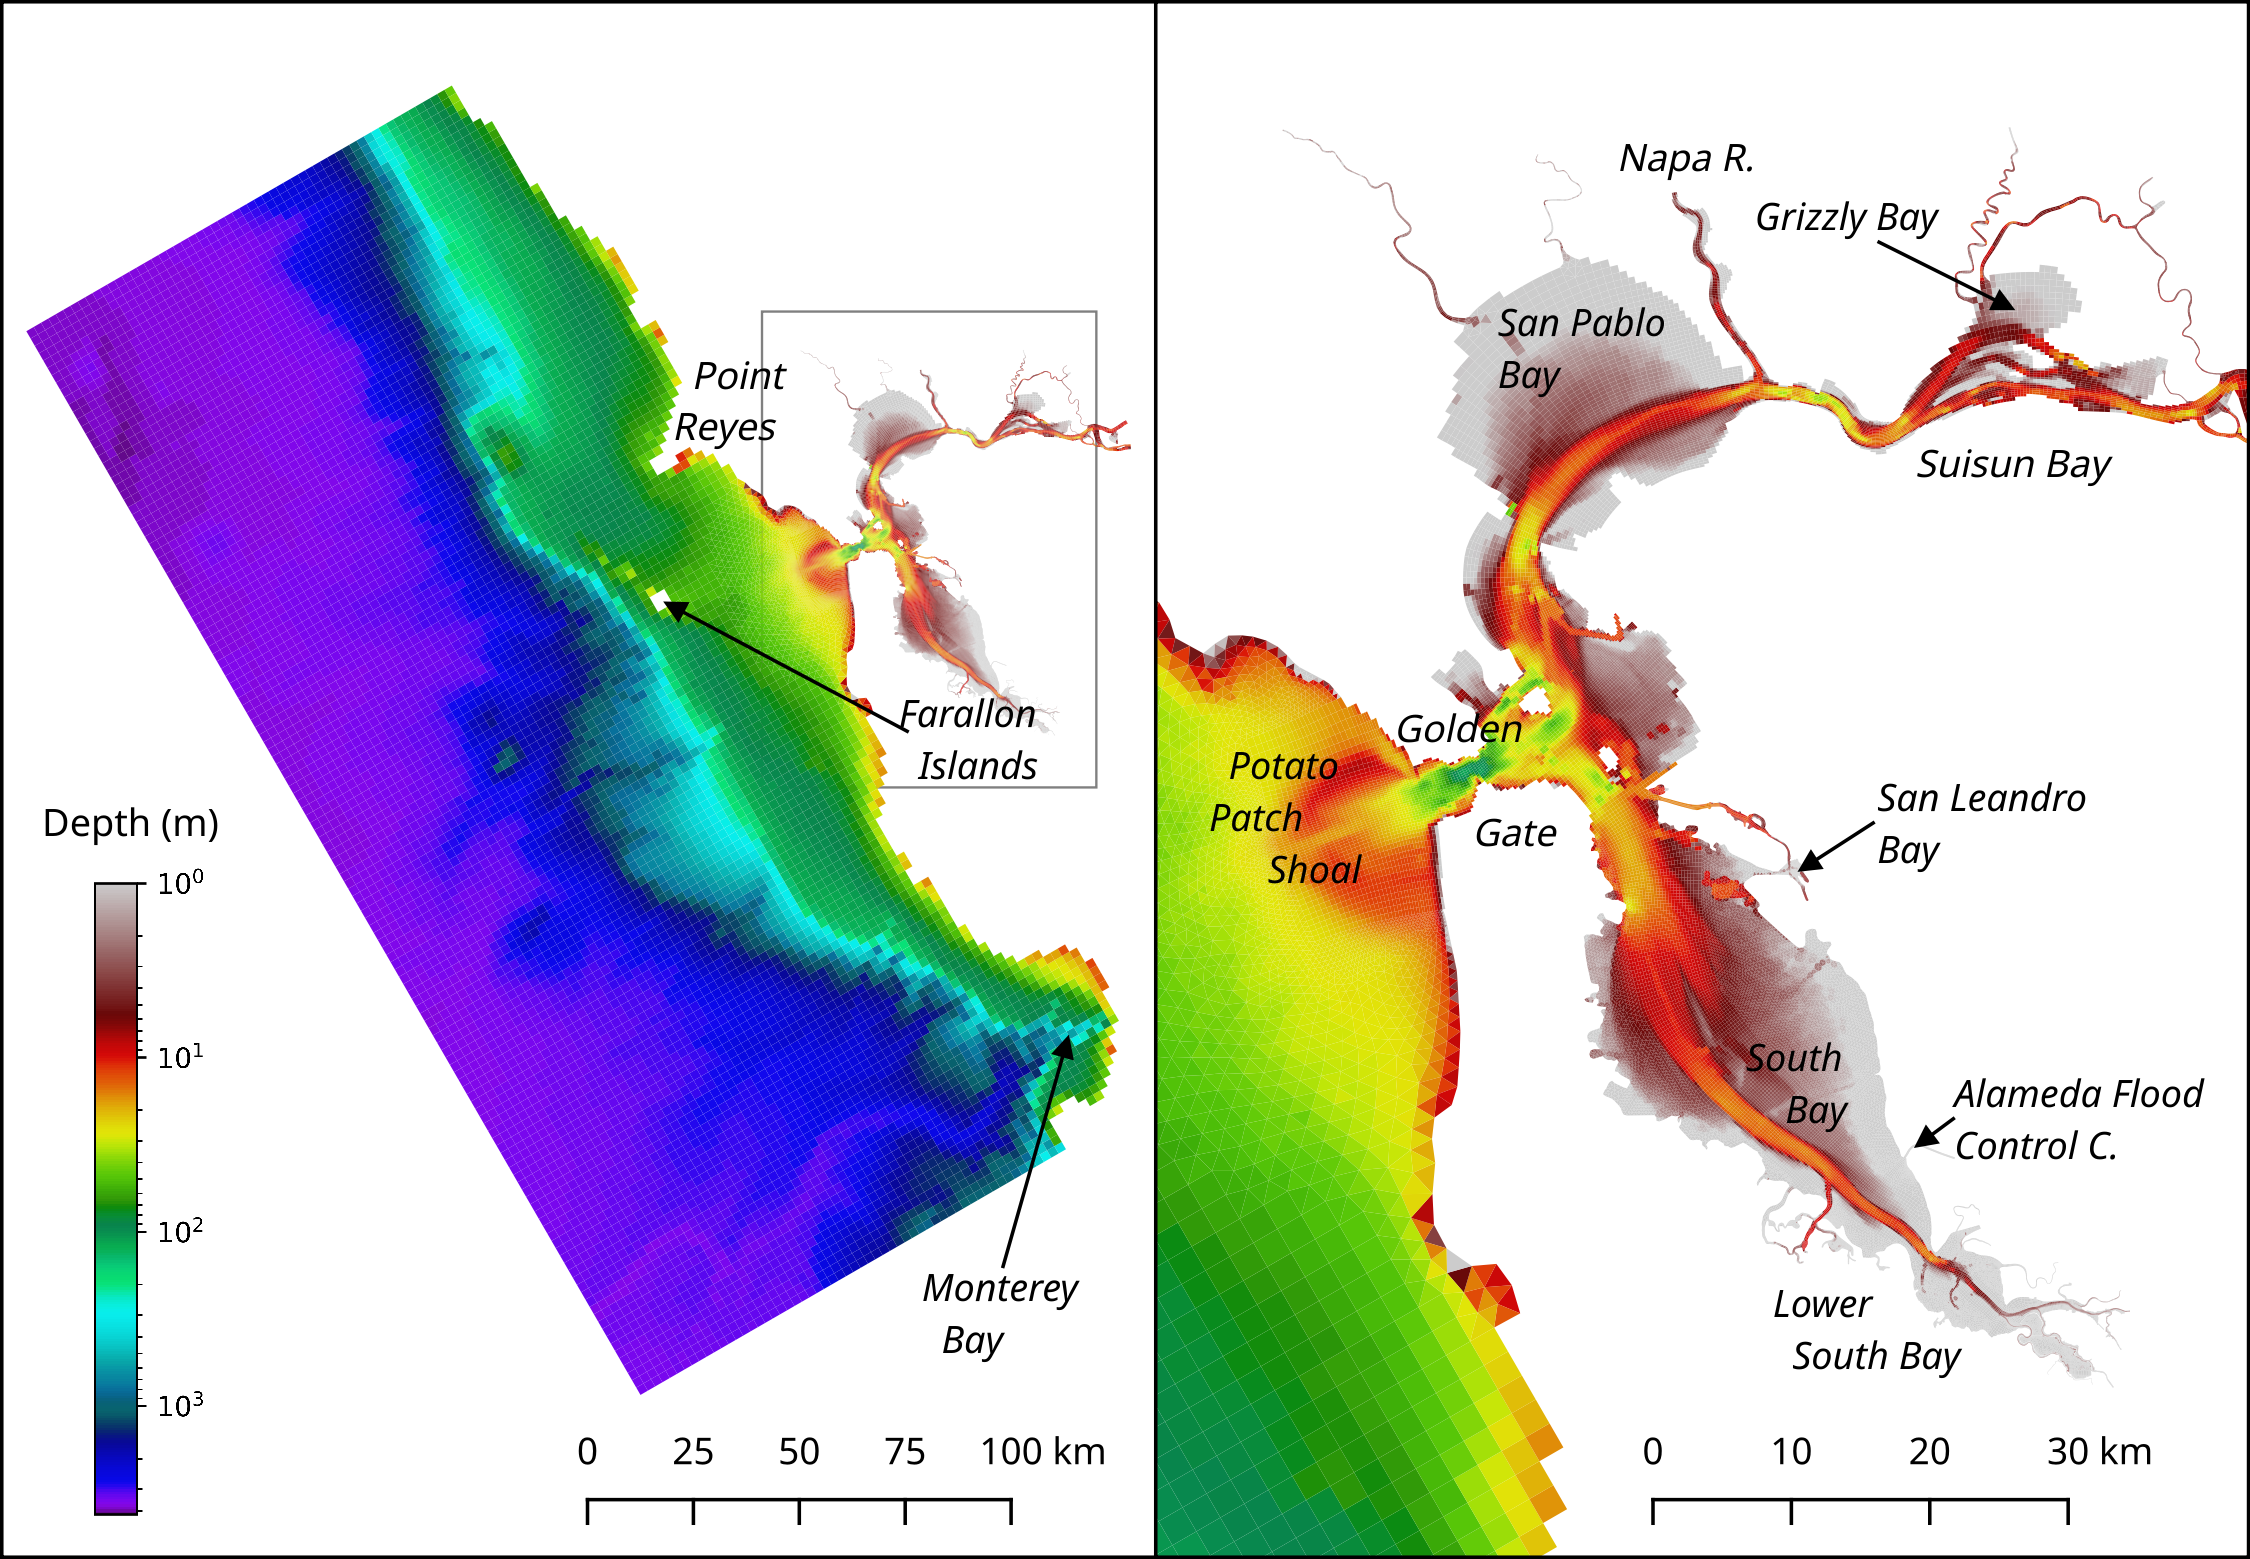
\includegraphics{figures/twopanel-overview.png}
  \caption{Hydrodynamic model domain}
  \label{model_domain}
\end{figure}

\begin{table}
  \caption{Model skill, water level}
  \label{model_skill}
  \centering
  \begin{tabular}{lrrr}
    \hline
        {} &  Amp & Lag (min) & Pearson \\
        Station      &      &           &         \\
        \hline
        Alameda      & 1.01 &     -14.2 &   0.984 \\
        Point Reyes  & 0.97 &     -19.0 &   0.978 \\
        Fort Point   & 0.98 &     -17.0 &   0.980 \\
        Coyote Creek & 0.91 &       1.3 &   0.984 \\
        Richmond     & 1.00 &     -17.4 &   0.980 \\
        Port Chicago & 1.29 &     -30.0 &   0.948 \\
        \hline
  \end{tabular}
\end{table}


\subsection{Particle Tracking Model}

The FISH-PTM offline particle tracking model \cite{Ketefian2015}
was used for integrating particle transport. All particles were
assigned a constant horizontal diffusion coefficient of
0.5~$\textrm{m}^2 \textrm{s}^{-1}$.  Each of the 8 sampled wastewater outfalls,
and the 15 largest stormwater sources were included as particle sources.
For each particle source, seven settling velocities were modeled: -0.05,
-0.005, -0.0005, 0, 0.0005, 0.005, and 0.05 ~$\textrm{m} \textrm{s}^{-1}$.
Each source/settling velocity combination had a constant 10 particles/hour
loading rate, and all particles were tracked for at least 20 days.
\marginnote{the runs are slow, but this seems like a very small
  number of particles}


\subsection{random quote from Ed re PTM and waves}

{\em from time scales special issue}

Other tracer-focused papers in this issue assessed or advanced
methodologies for measuring or modeling tracers or tracer-like
quantities. For example, Staneva et al. (2021) investigate processes
influencing particle transport by comparing different ocean-modeling
approaches to observations of physical drifters in the North
Sea. Specifically, those authors compare particle tracks computed with
a stand-alone ocean circulation model to those computed with the same
ocean circulation model coupled to a wave model, examining the
fidelity of each model set-up to observed drifter trajectories, as
well as high-frequency radar-based observations of current
velocity. It is shown that wave-induced drift significantly influences
particle transport in the upper layers of the ocean. This work
demonstrates that the coupling of circulation models to wave models
may greatly improve simulations of the transport of marine litter,
oil, larvae, or other biological materials.


\subsection{Particle Concentration Analysis}



\subsubsection{Blank Adjustment}

Field and laboratory blank samples revealed non-negligibile levels
of sample contamination in the various matrices.

\subsubsection{Loads}

\subsubsection{Ambient Concentrations}

\section{Results}


\subsection{Concentration in Central Bay}

{\em Hopefully this is actually borne out in the model}


\subsection{Loss from Surface}

Particle tracking results yielded the best correlation with and least
bias relative to surface trawl data when particles were removed from
the surface with a characteristic time scale of approximately two
days.  This loss time scale is on the short end of literature values
\marginnote{REFs}. Surface attrition is thought to occur through
combined processes of fragmentation and biofouling.  We compared size
distributions of particles in the Bay versus in the coastal ocean to
infer the relative importance of the two processes.  The underlying
assumptions are that Bay-sourced particles dominate any coastal
sources of particles, and that biofouling preferentially affects small
particles with large surface areas.  Figure \ref{surface_size_distributions}
shows histograms and associated kernel density estimates for the
major diameter of particles in surface water samples. The distributions
show that size distribution of fibers and fragments is unchanged as particles
move from the Bay to the ocean, while for films and foams the 
distribution shifts to larger lengths in the ocean. This
points to a winnowing of readily biofouled particles in the Bay, and on
a timescale that is not significantly longer than the Bay--coast transit time.

The comparison is not conclusive, though, and could also be explained
by the preferential transport of larger, more buoyant particles into the
coastal ocean as they ride nearer to the surface than marginally buoyant
particles.

\begin{figure}
  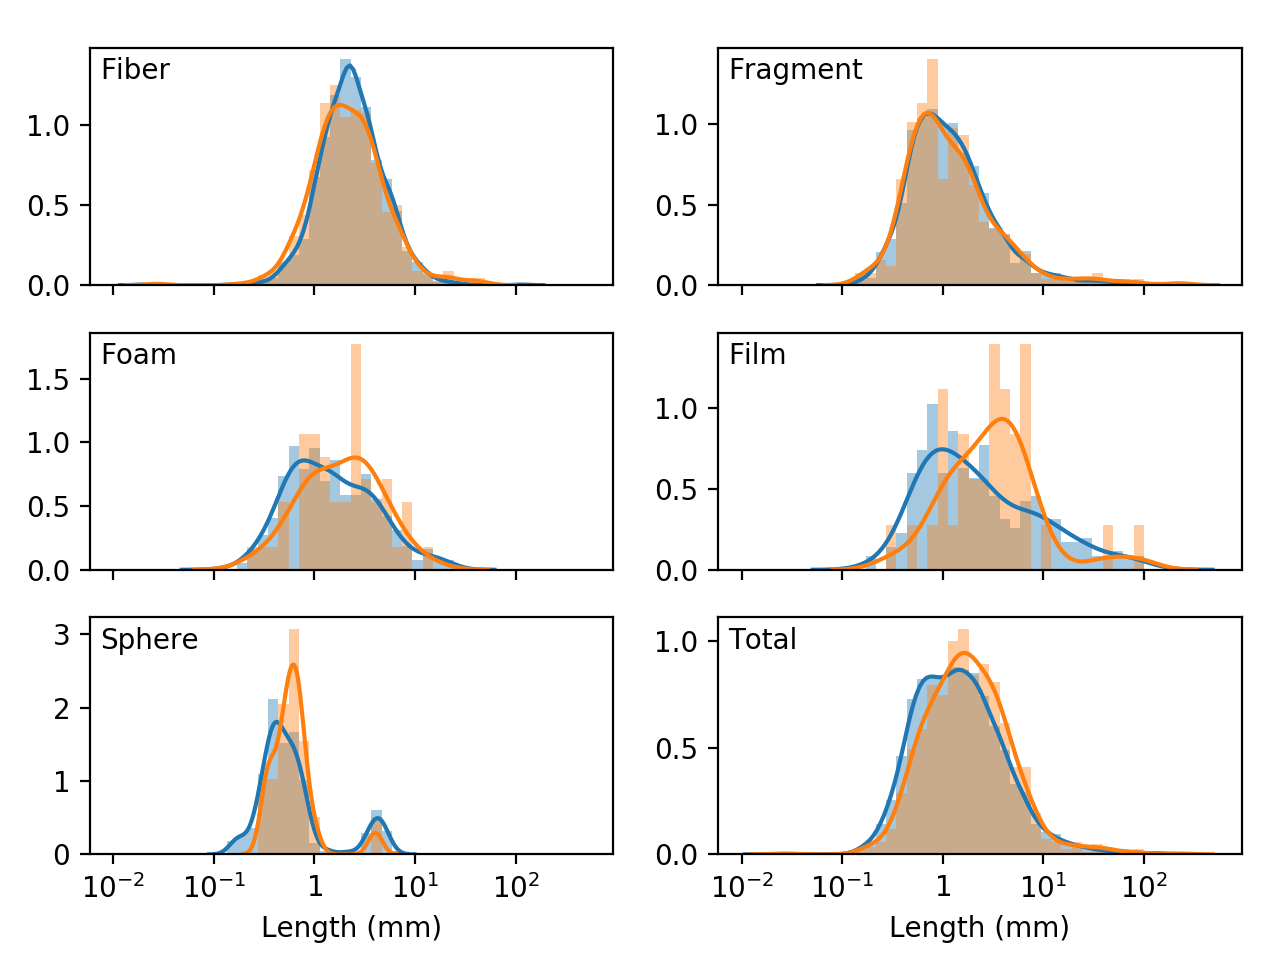
\includegraphics{figures/manta-bay_vs_coast-length_distribution.png}
  \caption{Particle length distributions from surface samples in the Bay and
    coastal ocean.}
  \label{surface_size_distributions}
\end{figure}

Validation ideas:
\begin{itemize}
  \item Alice reports greater concentrations in Central Bay surface
    water than in South Bay. Does the model capture this?
\end{itemize}


% recommended statement from
% https://www.hycom.org/publications/acknowledgements/hycom-data
Funding for the development of HYCOM has been provided by the National
Ocean Partnership Program and the Office of Naval Research. Data
assimilative products using HYCOM are funded by the
U.S. Navy. Computer time was made available by the DoD High
Performance Computing Modernization Program. The output is publicly
available at http://hycom.org.

%%

%  Numbered lines in equations:
%  To add line numbers to lines in equations,
%  \begin{linenomath*}
%  \begin{equation}
%  \end{equation}
%  \end{linenomath*}



%% Enter Figures and Tables near as possible to where they are first mentioned:
%
% DO NOT USE \psfrag or \subfigure commands.
%
% Figure captions go below the figure.
% Table titles go above tables;  other caption information
%  should be placed in last line of the table, using
% \multicolumn2l{$^a$ This is a table note.}
%
%----------------
% EXAMPLE FIGURES
%
% \begin{figure}
% \includegraphics{example.png}
% \caption{caption}
% \end{figure}
%
% Giving latex a width will help it to scale the figure properly. A simple trick is to use \textwidth. Try this if large figures run off the side of the page.
% \begin{figure}
% \noindent\includegraphics[width=\textwidth]{anothersample.png}
%\caption{caption}
%\label{pngfiguresample}
%\end{figure}
%
%
% If you get an error about an unknown bounding box, try specifying the width and height of the figure with the natwidth and natheight options. This is common when trying to add a PDF figure without pdflatex.
% \begin{figure}
% \noindent\includegraphics[natwidth=800px,natheight=600px]{samplefigure.pdf}
%\caption{caption}
%\label{pdffiguresample}
%\end{figure}
%
%
% PDFLatex does not seem to be able to process EPS figures. You may want to try the epstopdf package.
%

%
% ---------------
% EXAMPLE TABLE
%
% \begin{table}
% \caption{Time of the Transition Between Phase 1 and Phase 2$^{a}$}
% \centering
% \begin{tabular}{l c}
% \hline
%  Run  & Time (min)  \\
% \hline
%   $l1$  & 260   \\
%   $l2$  & 300   \\
%   $l3$  & 340   \\
%   $h1$  & 270   \\
%   $h2$  & 250   \\
%   $h3$  & 380   \\
%   $r1$  & 370   \\
%   $r2$  & 390   \\
% \hline
% \multicolumn{2}{l}{$^{a}$Footnote text here.}
% \end{tabular}
% \end{table}

%% SIDEWAYS FIGURE and TABLE
% AGU prefers the use of {sidewaystable} over {landscapetable} as it causes fewer problems.
%
% \begin{sidewaysfigure}
% \includegraphics[width=20pc]{figsamp}
% \caption{caption here}
% \label{newfig}
% \end{sidewaysfigure}
%
%  \begin{sidewaystable}
%  \caption{Caption here}
% \label{tab:signif_gap_clos}
%  \begin{tabular}{ccc}
% one&two&three\\
% four&five&six
%  \end{tabular}
%  \end{sidewaystable}

%% If using numbered lines, please surround equations with \begin{linenomath*}...\end{linenomath*}
%\begin{linenomath*}
%\begin{equation}
%y|{f} \sim g(m, \sigma),
%\end{equation}
%\end{linenomath*}

%%% End of body of article

%%%%%%%%%%%%%%%%%%%%%%%%%%%%%%%%
%% Optional Appendix goes here
%
% The \appendix command resets counters and redefines section heads
%
% After typing \appendix
%
%\section{Here Is Appendix Title}
% will show
% A: Here Is Appendix Title
%
%\appendix
%\section{Here is a sample appendix}

%%%%%%%%%%%%%%%%%%%%%%%%%%%%%%%%%%%%%%%%%%%%%%%%%%%%%%%%%%%%%%%%
%
% Optional Glossary, Notation or Acronym section goes here:
%
%%%%%%%%%%%%%%
% Glossary is only allowed in Reviews of Geophysics
%  \begin{glossary}
%  \term{Term}
%   Term Definition here
%  \term{Term}
%   Term Definition here
%  \term{Term}
%   Term Definition here
%  \end{glossary}

%
%%%%%%%%%%%%%%
% Acronyms
%   \begin{acronyms}
%   \acro{Acronym}
%   Definition here
%   \acro{EMOS}
%   Ensemble model output statistics
%   \acro{ECMWF}
%   Centre for Medium-Range Weather Forecasts
%   \end{acronyms}

%
%%%%%%%%%%%%%%
% Notation
%   \begin{notation}
%   \notation{$a+b$} Notation Definition here
%   \notation{$e=mc^2$}
%   Equation in German-born physicist Albert Einstein's theory of special
%  relativity that showed that the increased relativistic mass ($m$) of a
%  body comes from the energy of motion of the body—that is, its kinetic
%  energy ($E$)—divided by the speed of light squared ($c^2$).
%   \end{notation}




%%%%%%%%%%%%%%%%%%%%%%%%%%%%%%%%%%%%%%%%%%%%%%%%%%%%%%%%%%%%%%%%
%
%  ACKNOWLEDGMENTS
%
% The acknowledgments must list:
%
% >>>>	A statement that indicates to the reader where the data
% 	supporting the conclusions can be obtained (for example, in the
% 	references, tables, supporting information, and other databases).
%
% 	All funding sources related to this work from all authors
%
% 	Any real or perceived financial conflicts of interests for any
%	author
%
% 	Other affiliations for any author that may be perceived as
% 	having a conflict of interest with respect to the results of this
% 	paper.
%
%
% It is also the appropriate place to thank colleagues and other contributors.
% AGU does not normally allow dedications.


\acknowledgments
Enter acknowledgments, including your data availability statement, here.


%% ------------------------------------------------------------------------ %%
%% References and Citations

%%%%%%%%%%%%%%%%%%%%%%%%%%%%%%%%%%%%%%%%%%%%%%%
%
% \bibliography{<name of your .bib file>} don't specify the file extension
%
% don't specify bibliographystyle
%%%%%%%%%%%%%%%%%%%%%%%%%%%%%%%%%%%%%%%%%%%%%%%

\bibliography{references}



%Reference citation instructions and examples:
%
% Please use ONLY \cite and \citeA for reference citations.
% \cite for parenthetical references
% ...as shown in recent studies (Simpson et al., 2019)
% \citeA for in-text citations
% ...Simpson et al. (2019) have shown...
%
%
%...as shown by \citeA{jskilby}.
%...as shown by \citeA{lewin76}, \citeA{carson86}, \citeA{bartoldy02}, and \citeA{rinaldi03}.
%...has been shown \cite{jskilbye}.
%...has been shown \cite{lewin76,carson86,bartoldy02,rinaldi03}.
%... \cite <i.e.>[]{lewin76,carson86,bartoldy02,rinaldi03}.
%...has been shown by \cite <e.g.,>[and others]{lewin76}.
%
% apacite uses < > for prenotes and [ ] for postnotes
% DO NOT use other cite commands (e.g., \citet, \citep, \citeyear, \nocite, \citealp, etc.).
%



\end{document}



% More Information and Advice:

%% ------------------------------------------------------------------------ %%
%
%  SECTION HEADS
%
%% ------------------------------------------------------------------------ %%

% Capitalize the first letter of each word (except for
% prepositions, conjunctions, and articles that are
% three or fewer letters).

% AGU follows standard outline style; therefore, there cannot be a section 1 without
% a section 2, or a section 2.3.1 without a section 2.3.2.
% Please make sure your section numbers are balanced.
% ---------------
% Level 1 head
%
% Use the \section{} command to identify level 1 heads;
% type the appropriate head wording between the curly
% brackets, as shown below.
%
%An example:
%\section{Level 1 Head: Introduction}
%
% ---------------
% Level 2 head
%
% Use the \subsection{} command to identify level 2 heads.
%An example:
%\subsection{Level 2 Head}
%
% ---------------
% Level 3 head
%
% Use the \subsubsection{} command to identify level 3 heads
%An example:
%\subsubsection{Level 3 Head}
%
%---------------
% Level 4 head
%
% Use the \subsubsubsection{} command to identify level 3 heads
% An example:
%\subsubsubsection{Level 4 Head} An example.
%
%% ------------------------------------------------------------------------ %%
%
%  IN-TEXT LISTS
%
%% ------------------------------------------------------------------------ %%
%
% Do not use bulleted lists; enumerated lists are okay.
% \begin{enumerate}
% \item
% \item
% \item
% \end{enumerate}
%
%% ------------------------------------------------------------------------ %%
%
%  EQUATIONS
%
%% ------------------------------------------------------------------------ %%

% Single-line equations are centered.
% Equation arrays will appear left-aligned.

Math coded inside display math mode \[ ...\]
 will not be numbered, e.g.,:
 \[ x^2=y^2 + z^2\]

 Math coded inside \begin{equation} and \end{equation} will
 be automatically numbered, e.g.,:
 \begin{equation}
 x^2=y^2 + z^2
 \end{equation}


% To create multiline equations, use the
% \begin{eqnarray} and \end{eqnarray} environment
% as demonstrated below.
\begin{eqnarray}
  x_{1} & = & (x - x_{0}) \cos \Theta \nonumber \\
        && + (y - y_{0}) \sin \Theta  \nonumber \\
  y_{1} & = & -(x - x_{0}) \sin \Theta \nonumber \\
        && + (y - y_{0}) \cos \Theta.
\end{eqnarray}

%If you don't want an equation number, use the star form:
%\begin{eqnarray*}...\end{eqnarray*}

% Break each line at a sign of operation
% (+, -, etc.) if possible, with the sign of operation
% on the new line.

% Indent second and subsequent lines to align with
% the first character following the equal sign on the
% first line.

% Use an \hspace{} command to insert horizontal space
% into your equation if necessary. Place an appropriate
% unit of measure between the curly braces, e.g.
% \hspace{1in}; you may have to experiment to achieve
% the correct amount of space.


%% ------------------------------------------------------------------------ %%
%
%  EQUATION NUMBERING: COUNTER
%
%% ------------------------------------------------------------------------ %%

% You may change equation numbering by resetting
% the equation counter or by explicitly numbering
% an equation.

% To explicitly number an equation, type \eqnum{}
% (with the desired number between the brackets)
% after the \begin{equation} or \begin{eqnarray}
% command.  The \eqnum{} command will affect only
% the equation it appears with; LaTeX will number
% any equations appearing later in the manuscript
% according to the equation counter.
%

% If you have a multiline equation that needs only
% one equation number, use a \nonumber command in
% front of the double backslashes (\\) as shown in
% the multiline equation above.

% If you are using line numbers, remember to surround
% equations with \begin{linenomath*}...\end{linenomath*}

%  To add line numbers to lines in equations:
%  \begin{linenomath*}
%  \begin{equation}
%  \end{equation}
%  \end{linenomath*}



